%!TEX TS-program = xelatex 
\documentclass[aspectratio=1610,xcolor=dvipsnames,t,compress]{beamer} 

\usepackage{listings} 
\usepackage{color} 
\usepackage{xcolor}  
\usepackage{microtype} 
\usepackage{helvet} 
\usepackage{inconsolata} 
\usepackage[framemethod=TikZ]{mdframed} 
\usepackage{graphicx} 
\usepackage{alltt}
\usepackage{sverb} 
\usepackage{verbatim} 
\usepackage{pifont} 
\usepackage{helvet} 
\usepackage{algorithm}
\usepackage{algpseudocode}

\usetheme[noflama]{sthlm}

%\usetheme{Madrid} 
%\useoutertheme{smoothbars} 
\useinnertheme{rectangles} 

\setbeamertemplate{navigation symbols}{}
\setbeamertemplate{blocks}[default] 

%\definecolor{mypurple}{rgb}{.49,0,98}
%\setbeamercolor*{palette primary}{use=structure,fg=white,bg=green}
%\usecolortheme[rgb={0.9,0.2,0.2}]{structure}
%\usecolortheme[rgb={0.6,0.1,0.1}]{structure}

%\usecolortheme[rgb={0.2, 0.2, 0.8}]{structure} 
\usecolortheme[rgb={0.0, 0.0, 0.8}]{structure} 

\usepackage{color}
\definecolor{orange}{cmyk}{0,0.4,0.8,0.2}
\definecolor{darkorange}{rgb}{.71,0.21,0.01}
\definecolor{darkgreen}{rgb}{.12,.54,.11}
\definecolor{myteal}{rgb}{.26, .44, .56}
\definecolor{gray}{gray}{0.45}
\definecolor{lightgray}{gray}{.95}
\definecolor{mediumgray}{gray}{.8}
\definecolor{inputbackground}{rgb}{.95, .95, .85}
\definecolor{outputbackground}{rgb}{.95, .95, .95}
\definecolor{traceback}{rgb}{1, .95, .95}
\definecolor{inputbg}{rgb}{0.98, 0.98, 0.98}

\usepackage{listings} 
\lstset{language=bash,
        %basicstyle=\footnotesize\ttfamily, 
        basicstyle=\small\ttfamily,
        columns=fullflexible, 
        %title=\lstname, 
        %numbers=left, stringstyle=\texttt, 
        %numberstyle={\tiny\texttt}, 
        keywordstyle=\color{blue}, 
        commentstyle=\color{darkgreen}, 
        stringstyle=\color{purple} } 


\mdfsetup{skipabove=\topskip, skipbelow=\topskip} 

\definecolor{codebg}{rgb}{0.99,0.99,0.99}

\global\mdfdefinestyle{code}{%
    frametitlerule=true,%
    frametitlefont=\small\bfseries\ttfamily,%
    frametitlebackgroundcolor=lightgray,%
    backgroundcolor=codebg,%
    linecolor=gray, linewidth=0.5pt,%
    leftmargin=0.5cm, rightmargin=0.5cm,%
    roundcorner=2pt,%
    innerleftmargin=5pt
}

\global\mdfdefinestyle{code2}{%
    topline=false,%
    bottomline=false,%
    leftline=true,%
    rightline=false,%
    backgroundcolor=codebg,%
    linecolor=gray, linewidth=0.5pt,%
    leftmargin=0.0cm, rightmargin=0.0cm,%
    innerleftmargin=1pt
}

\newcommand{\showcode}[1]{\begin{mdframed}[style=code] %
                            \lstinputlisting{#1}% 
                          \end{mdframed}% 
}

%\title[Software Engineering]{Software Architecture and Architectural Design} 
\title[Software Engineering]{Detailed Design with UML} 
\subtitle{Software Engineering Process and Practice} 
\author[Michael Papasimeon]{Dr Michael Papasimeon} 
\date{18 May 2003} 

\begin{document}

\begin{frame}
    \maketitle
\end{frame} 

\begin{frame}{Overview}
    \begin{itemize}
        \item Class Diagrams
        \item Inheritance and Abstract Classes
        \item Attributes and Associations
        \item Roles
        \item Aggregation and Composition
        \item Association Multiplicity
        \item Qualified Associations
        \item Programmer Notes
    \end{itemize}
\end{frame}

\begin{frame}{UML Class Diagrams}
    \begin{center}
        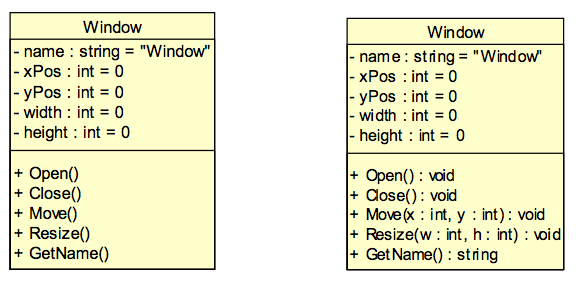
\includegraphics[width=0.6\textwidth]{images/window} 
    \end{center} 
\end{frame}

\begin{frame}{Attribute and Method Visibility} 
    Attributes and methods can be prefixed with symbols to denote if they are
    private, protected or public. 
    \begin{itemize}
        \item \texttt{-} Private
        \item \texttt{\#} Protected
        \item \texttt{+} Public
    \end{itemize}
\end{frame} 

\begin{frame}{Inheritance and Abstract Classes} 
    \begin{center}
        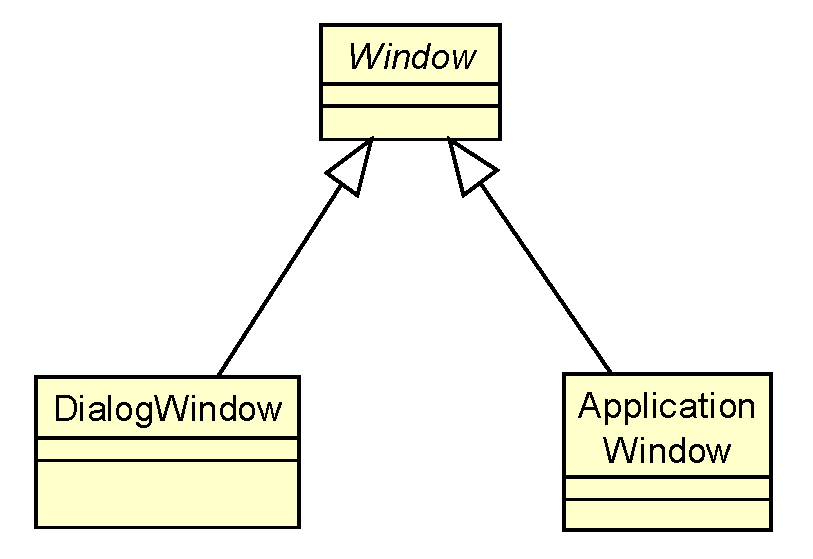
\includegraphics[width=0.6\textwidth]{images/inheritance} 
    \end{center} 
\end{frame} 

\begin{frame}{Attributes and Associations} 
    \begin{center}
        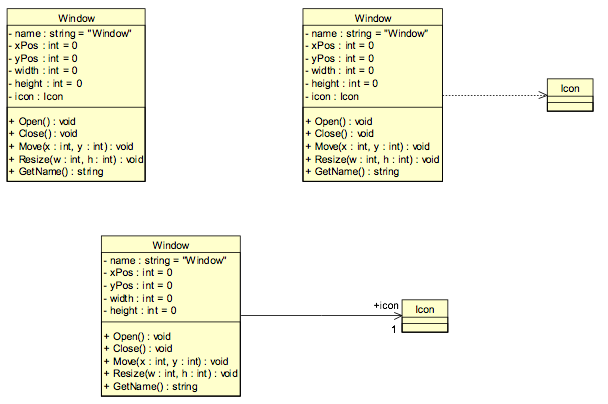
\includegraphics[width=0.8\textwidth]{images/attributes} 
    \end{center} 
\end{frame} 

\begin{frame}{Associations} 
    \begin{center}
        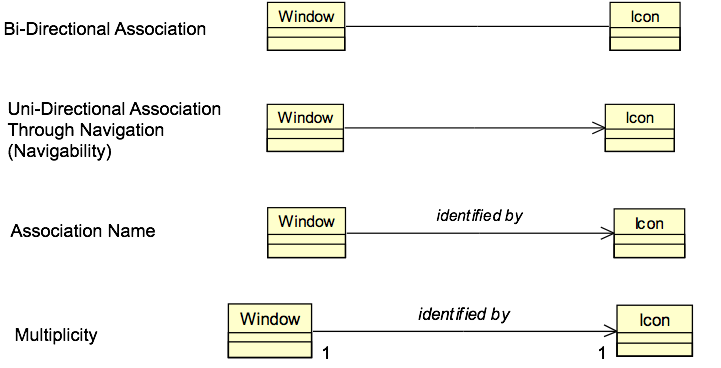
\includegraphics[width=0.8\textwidth]{images/associations} 
    \end{center} 
\end{frame} 

\begin{frame}{Association Roles}  
    \begin{center}
        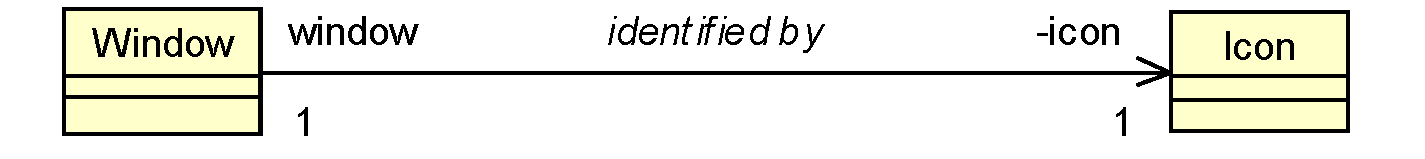
\includegraphics[width=0.8\textwidth]{images/roles} 
    \end{center} 
\end{frame}

\begin{frame}{Aggregation and Composition} 
    \begin{center}
        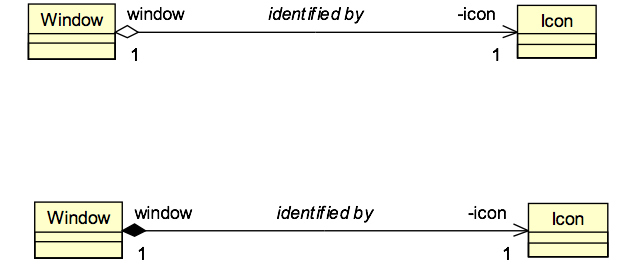
\includegraphics[width=0.8\textwidth]{images/aggregation} 
    \end{center} 
\end{frame} 

\begin{frame}{Multiplicities in Associations} 
    \begin{center}
        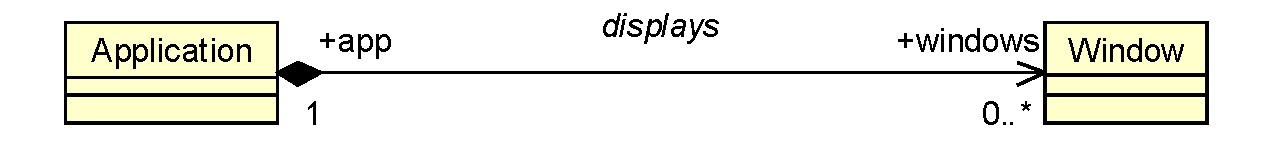
\includegraphics[width=0.8\textwidth]{images/multiplicity} 
    \end{center} 
\end{frame} 

\begin{frame}{Qualified Associations}
    \begin{center}
        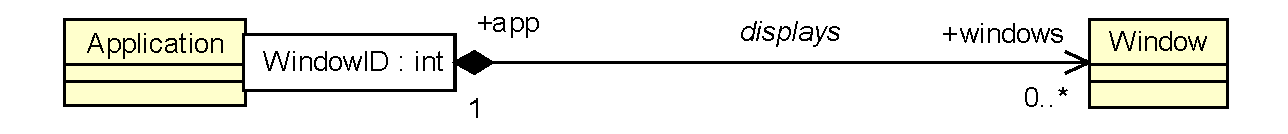
\includegraphics[width=0.8\textwidth]{images/qualified} 
    \end{center} 
\end{frame}

\begin{frame}{Notes for the Programmer} 
    \begin{center}
        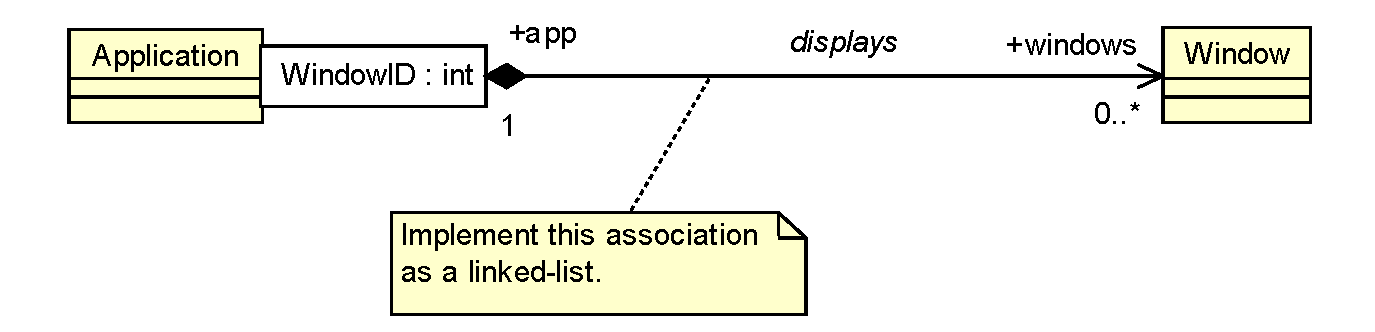
\includegraphics[width=0.8\textwidth]{images/notes} 
    \end{center} 
\end{frame} 

\end{document}
